\chapter{Software In The Loop Testing}
When working with UAVs safety is a critical issue. To be able to verify software before test flights is of great importance and will make a much simpler workflow. This chapter will go through the setup of the software in the loop (SITL) test. And explain how the different systems are interfaced to each other. The different SITL-test conducted will also be presented.
\section{SITL-Setup}
The main purpose of the SITL-test is to verify the control software presented in Chapter \ref{control_SW}.\\
\newline
The SITL-setup contains of six main components. These components are DUNE, Neptus, ArduCopter SITL, ArduPilot, MAVProxy and APM Planner. These have different functions, and not all of them are necessary. The interface between the different components is displayed in Figure \ref{sitl}, and their roles are briefly explained below.
\begin{figure}[H]
\centering
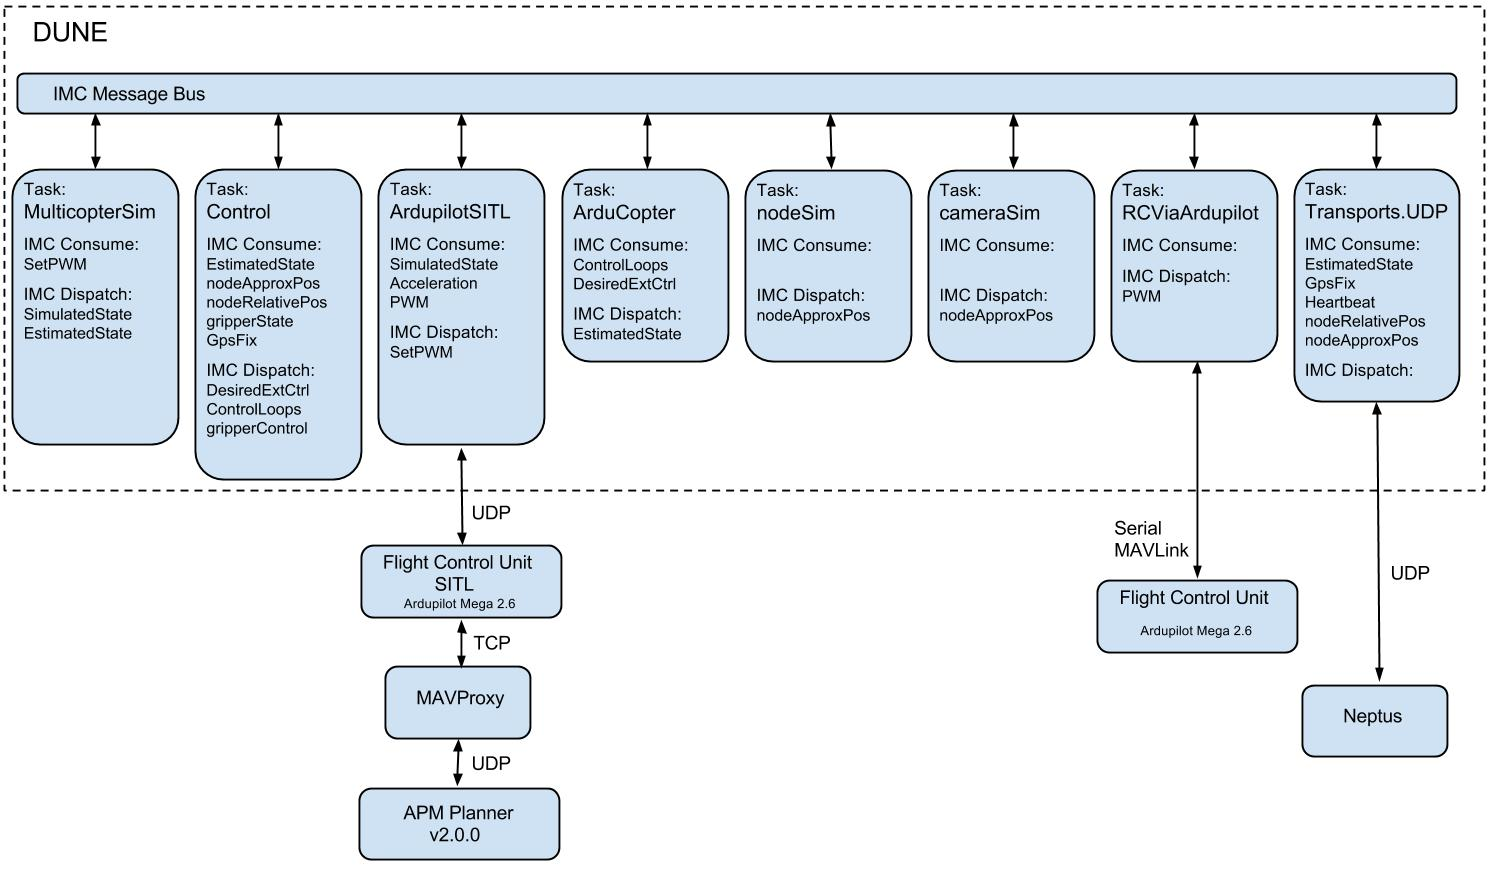
\includegraphics[width = 17cm]{fig/Simulation.jpg}
\caption{Setup used for SITL-testing}
\label{sitl}
\end{figure}
\subsubsection*{DUNE}
DUNE is the part of the SITL that is put to the test. To be able to see if the control algorithms work. Some of the features needs to be simulated. This is done in Task that only are run in SITL mode. A model of a multicopter is used to calculate realistic attitude and position states based of the actuator inputs given to the Task. There is another Task that  
\subsubsection*{Neptus}
Neptus is used to monitor values of the relevant IMC-messages. It is used in exactly the same way that it is used in real missions.
\subsubsection*{ArduCopter SITL}
The ArduCopter project contains a SITL-feature. This means that one can choose to compile the project for SITL instead of for use with hardware. This feature is very practical both for testing changes done to the ArduCopter project and to test the way DUNE and ArduCopter interface each other. The ArduCopter code has been altered by the hexacopter team at AMOS to include a DUNE mode. This mode is verified using the SITL feature.
\subsubsection*{ArduPilot}
To be able to test manual control in the SITL setup, ArduPilot hardware (running ArduCopter code) is included to send PWM values from a radio into the SITL.
\subsubsection*{MAVProxy}
MAVProxy is a simple ground control station, but it is not used for that in this setup. The task for MAVProxy here is simply to be a bridge between the ArduCopter SITL and AMP Planner, which is another ground control station. This bridge is needed because the ArduCopter SITL use TCP to emulate a serial port used for communication while APM Planner connects using UDP.
\subsubsection*{APM Planner}
APM Planner is a very versatile ground control station developed as an open source project. The version used in this setup is an altered version developed by the hexacopter group at AMOS to include DUNE mode. It is convenient to use this ground control station because it gives easy access to state values at the AarduCopter SITL and an simple interface to modify parameters used by the ArduCopter SITL. It can also be used to arm the ArduCopter SITL and to change mode.
\section{Some test 1}
\section{Some test 2}
\section{Results}